%
\section{Entire System Integration}

To insure that all parts work, it is needed to connect them all to one software mechanism or control flow going through one point. Another design could be multi-agent systems (MAS) where all software will be separate agent.

The Sorting algorithm, RFID reader, MySQL Library, socket transfer server are connected:

\begin{figure}[h]
	\centering
		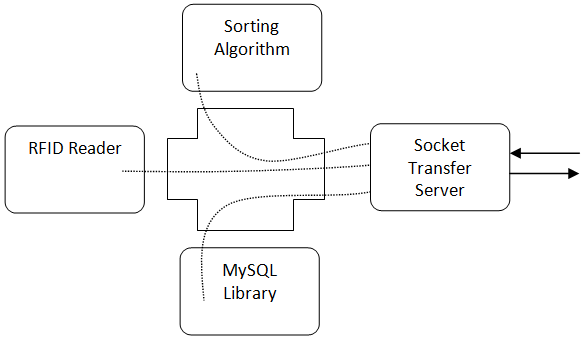
\includegraphics[scale=0.6]{softwareInteraction}
	\caption{Interaction between the different elements}
	\label{fig:softwareInteraction}
\end{figure}


\subsection{Tests/Analysis/Functionality}

\begin{table}[h]
	
    \begin{tabular}{ | p{0.5cm} | p{3.8cm} |p{1cm} |}
    \hline
	No & Modules & Total\\ \hline
	1 & Database & 100\% \\ \hline
	2 & MySQL library &  90\% \\ \hline
	3 & Socket Transfer server &  100\% \\ \hline
	4 & RFID reader &  100\% \\ \hline
	5 & Sorting Algorithm &  100\% \\ \hline
    \end{tabular}
	\caption{Estimation in percents of current system}
	\label{tab:percentSystem}
\end{table}

\begin{enumerate}
	\item Database function very well, no errors during period
	\item MySQL library function very well, however some exceptions occured during the project period. Problems with MySQL connector library. Assumption that exceptions come when some one tries to change database during usage or it can be problems with multithreading. They were reported by subtask 6. We do not think this will be a big problem.
	\item Socket transfer server functions 100\%.
	\item RFID reader works for this subtasks usage, it were not tested extensively by us, because it is a library that is provided by subtask 6.
	\item Sorting algorithm seem to work ok, however it is not tested 100\% due to time constraints.
\end{enumerate}

\subsection{Future Work}
A webserver could be a nice feature to add to provide some information about the elders clothes, where they are in the washing process and to get an estimated time of arrival to the rest home. Another feature that is not implemented is a picture of the elder that is the owner of the clothes, this could also be stored on the webserver.

\begin{figure}[h]
	\centering
		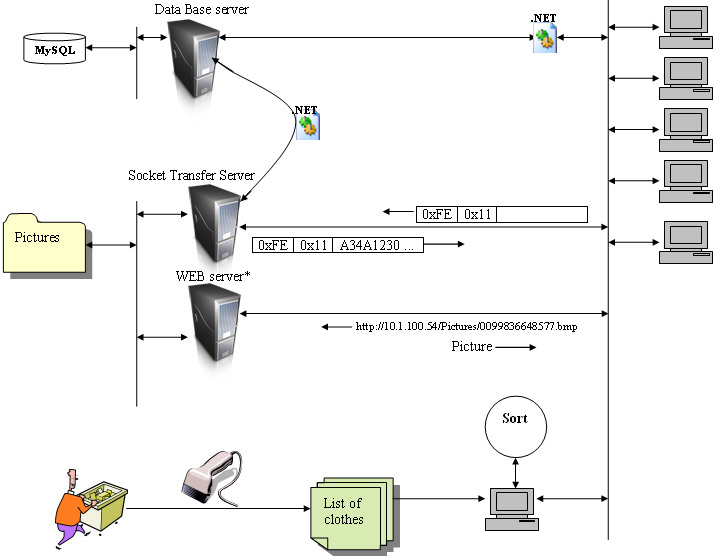
\includegraphics[scale=0.5]{entireSystem}
	\caption{Future System}
	\label{fig:entireSystem}
\end{figure}